\documentclass[11pt,a4paper,oneside,onecolumn]{scrartcl}

\usepackage[ngerman]{babel}			% deutschsprachiger Textsatz
\usepackage[utf8]{inputenc}			% Eingabekodierung
\usepackage[T1]{fontenc}			% Schriftenkodierung
\usepackage{graphicx}				% Einbinden von Grafiken
\usepackage{lmodern}				% Ersatz für Computer Modern-Schriften
\usepackage{amsmath}				% Mathematische Symbole
\usepackage{stmaryrd}
\usepackage{listings}				% Syntax highlighting
\usepackage{amssymb}				% Noch mehr mathematische Symbole
\usepackage{amsfonts}				% Schriften für mathematischen Formelsatz
\usepackage{url}					% Zur Darstellung von URLs im Dokument
\usepackage[small,bf]{caption}
\usepackage{array}


\setlength{\captionmargin}{11pt}	% auf Schriftgröße anzupassen

\pagestyle{myheadings}
\markright{Pathfinding}
 
\date{\normalsize{\today}}

\begin{document}
%\maketitle
%\tableofcontents



%\newpage
\section*{Pathfinding}
\subsection*{Überblick}
	Im folgenden wird der Pathfinding Algorithmus nähr beschrieben bei welchem aus einer erkundenten Karte und einem Start und Zielpunkt ein optimaler Pfad berechnet wird. Bedingungen hierfür sind jedoch eine erkundete Topologie. Übergeben wird diese als binährer 2-Dimensionaler Array, sowie einem Startpunkt des Naos und dem gefundenen Endpunkt. Der Algorithmus teilt sich in 3 Phasen: 1. Die Breitensuche, die dafür sorgt ein gültigen Pfad vom Start, zum Endpunkt zu finden. 2. Die Repositionierung des Pfades um ein möglichst großen Abstand zu den Hindernissen zu erreichen. 3 Die Pfadoptimierung, die eine Minimierung der Punkte zum Ziel hat. Das Resultat ist ein optimierter Pfad vom Start, zum Zielpunkt. Repräsentiert wird dieser durch eine Liste von Punkten.
\subsection*{1. Breitensuche}
	Bei der Representation der Karte handelt es sich um ein 2-Deminsionallen Binären Array, wobei 1 für ein Hindernis stehen und 0 für einen Freifläche. Die Breitensuche geht nun folgendermaßen vor: Sie weist iterativ jedem Punkt die Entfernung zum Startpunkt zu. Dies geschieht indem jeder Punkt am Horizont, also der noch nicht betrachtet wurde und an einen bereits betrachteten Punkt grenzt, den Abstand des bisherigen Punktes + 1 annimmt. Dies geschieht so lange der Endpunkt noch nicht gefunden wurde. Ist ein Endpunkt gefunden Konstruiert man den Pfad vom Endpunkt zum Startpunkt aus, in dem jeweils immer der kleinste Folgepunkt dem Pfad hinzugefügt wird, bis man bei dem Startpunkt angekommen ist. Das Resultat ist ein Pfad an Punkten.\\
	\\
	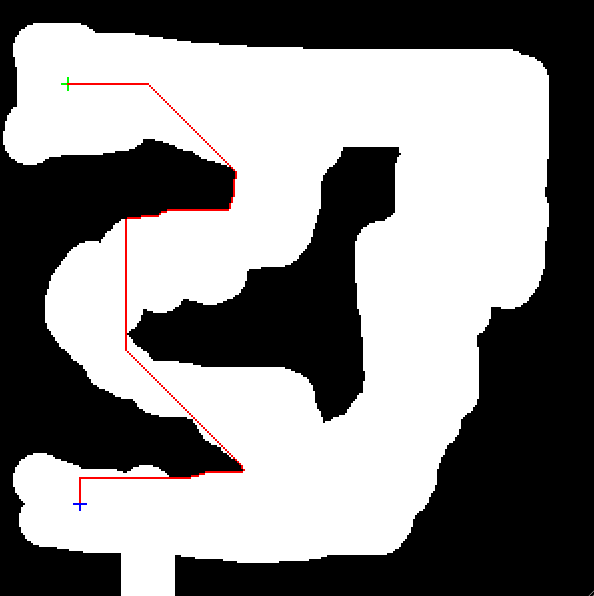
\includegraphics[scale=0.45]{p2.png} 
\subsection*{2. Repositioniertung}
	Die Breitensuche sollte nun einen Pfad zurückliefern. Dieser Pfad ist jedoch auf die minimale Distanz optimiert. Einen Roboter entlang dieses Pfades zu schicken ist nicht möglich, da der Pfad oft an möglichen Hindernissen langführt und die Breite der Roboter nicht berücksichtigt. Da die Position der Hindernisse auf der Karte auch einem Fehler unterliegen ist es sicherer den Roboter in der "Mitte" eines "Ganges" zu schicken. Die Repositionierung sträbt nun an aus dem Pfad der Breitensuche einen solchen optimalen Pfad an, der möglichst weit weg von möglichen hindernissen ist. Dazu wird durch jeden Punkt des Pfades 4 Linien geführt: Die Horizontale, Vertikale und beide Diagonalen, die jewels dort enden, wo diese an ein mögliches Hindernis stoßen. Um eine Abschätzung des Optimalen Punktes zu bekommen, wird nun der Mittelpunkt der kürzisten Linie genommen und aus ihr wird ein Kreis mit der Diagonale der Linie konstruiert. Das Ergebnis ist eine Menge M von Kreisen auf der Karte. \\

	\\
	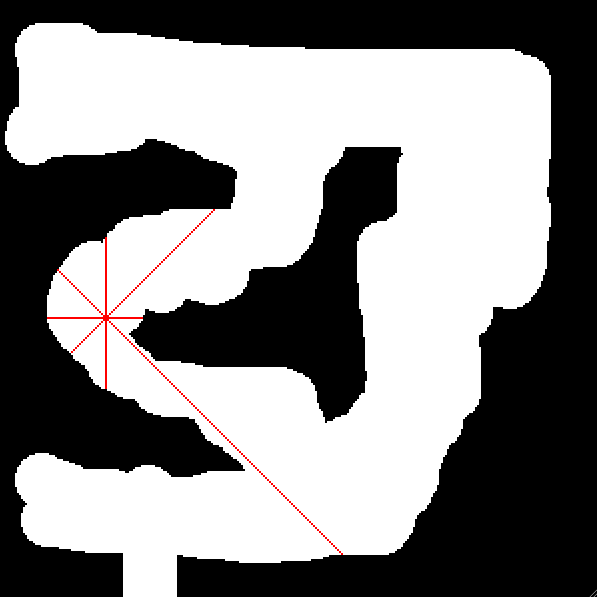
\includegraphics[scale=0.45]{p3.png} \\ \\
	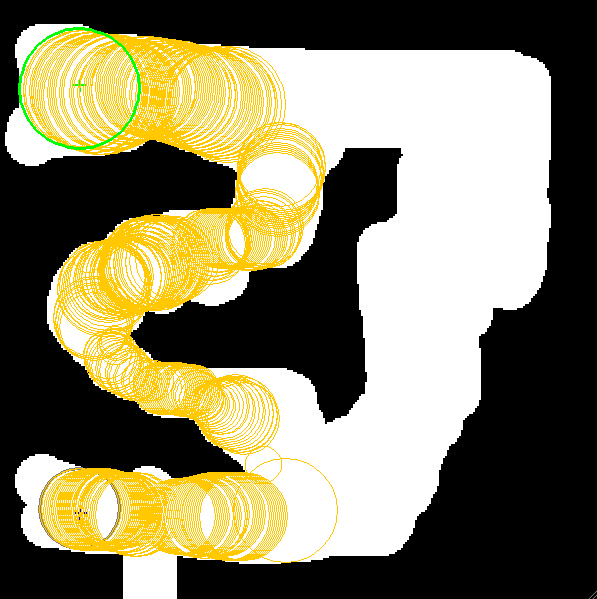
\includegraphics[scale=0.45]{p4.png} 

\subsection*{3. Optimierung}
	In der Optimierungsphase werden alle Kreise aus M, die sich überschneiden, miteinander verbunden. Das Ergebnis ist ein Graph. Auf dem resultierendem Graphen wird nun noch einmal eine Breitensuche vorgenommen, wobei die Länge der Verbindung mit einberechnet wird. Der resultierende Pfad aus dieser Breitensuche ist der gesuchte Pfad und wird zurückgegeben. \\
	\\
	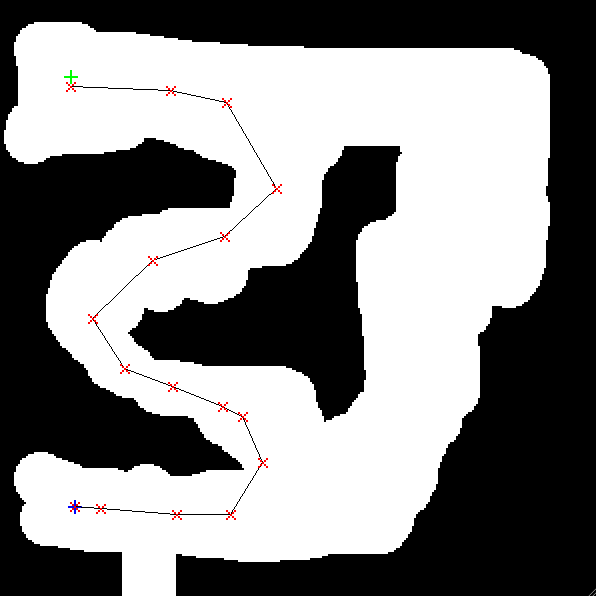
\includegraphics[scale=0.45]{p5.png} 

\end{document}

